% This file is part of Oaklisp.
%
% This program is free software; you can redistribute it and/or modify
% it under the terms of the GNU General Public License as published by
% the Free Software Foundation; either version 2 of the License, or
% (at your option) any later version.
%
% This program is distributed in the hope that it will be useful,
% but WITHOUT ANY WARRANTY; without even the implied warranty of
% MERCHANTABILITY or FITNESS FOR A PARTICULAR PURPOSE.  See the
% GNU General Public License for more details.
%
% The GNU GPL is available at http://www.gnu.org/licenses/gpl.html
% or from the Free Software Foundation, 59 Temple Place - Suite 330,
% Boston, MA 02111-1307, USA

\documentclass[12pt]{report}
\usepackage{times}
\usepackage{fullpage}
\usepackage{graphicx}
\usepackage{makeidx}
\usepackage[numbers]{natbib}
\usepackage[hyphens]{url}
\urlstyle{same}

\makeindex

\begin{document}


\bibliographystyle{plain}

% \newcommand{\comment}[1]{}
\newcommand{\df}[1]{{\tt#1}\index{{\tt#1}}}
\newcommand{\dffl}[1]{{\tt(fluid #1)}\index{{\tt#1} ! fluid}}
\newcommand{\dfcoer}[1]{{\tt(coercer #1)}\index{{\tt#1} ! coercer}}
\newcommand{\dfsw}[1]{{\tt#1}\index{{\tt#1} ! switch}}

\newenvironment{docenv}{\nopagebreak\vspace{-4ex}\nopagebreak
\begin{quotation}\noindent}{\end{quotation}}

\newcommand{\doc}[1]{\nopagebreak\vspace{-4ex}\nopagebreak
\begin{quotation}\noindent#1\end{quotation}}

\newcommand{\discbar}{\rule{3in}{.2mm}}
\newenvironment{discussenv}{\begin{quote}\begin{quote}\discbar\par}{\par\discbar\end{quote}\end{quote}}
\newcommand{\discuss}[1]{\begin{discussenv}#1\end{discussenv}}

\newcommand{\macdef}[2]{{\tt#1}\ \meq\ {\tt#2}\newline}
\newcommand{\evto}[2]{{\tt#1}\ \ra\ {\tt#2}}

\newcommand{\header}[2]{\par\noindent\hspace{\leftmargini
}{#1}\hfill{\em#2}\hspace*{\leftmargini}\newline}
\newcommand{\heady}[3]{\index{{\tt#1} ! #3}\header{{\tt#1 \em#2}}{#3}}
\newcommand{\headyy}[3]{\index{{\tt#1} ! #3}\header{{\tt(#1 \em#2\tt)}}{#3}}

\newcommand{\sform}[2]{\headyy{#1}{#2}{Special Form}}
\newcommand{\op}[2]{\headyy{#1}{#2}{Operation}}
\newcommand{\so}[2]{\headyy{#1}{#2}{Settable Operation}}
\newcommand{\lo}[2]{\headyy{#1}{#2}{Locatable Operation}}
\newcommand{\mc}[2]{\headyy{#1}{#2}{Macro}}

\newcommand{\fn}[2]{\headyy{#1}{#2}{Function}}
\newcommand{\pr}[2]{\headyy{#1}{#2}{Predicate}}
\newcommand{\spred}[2]{\headyy{#1}{#2}{Settable Predicate}}

\newcommand{\gv}[1]{\heady{#1}{}{Global Variable}}
\newcommand{\ob}[1]{\heady{#1}{}{Object}}
\newcommand{\ty}[1]{\heady{#1}{}{Type}}
\newcommand{\cty}[1]{\heady{#1}{}{Coercable Type}}
\newcommand{\fv}[1]{\index{{\tt#1} ! Fluid Variable}\header{\tt (fluid
#1)}{Fluid Variable}}

\newcommand{\makin}[2]{\index{{\tt#1} ! Making}\header{\tt (make #1
\em#2\tt)}{Operation}}
\newcommand{\setter}[3]{\index{{\tt#1} ! Setter}\header{\tt(set! (#1
\em#2\tt) \em#3\tt)}{Operation}}
\newcommand{\coercer}[2]{\index{{\tt#1} ! Coercer}\header{\tt((coercer
#1) \em#2\tt)}{Coarcable Type}}
\newcommand{\oop}[1]{\index{{\tt#1} ! Operation}\header{\tt(#1)}{Operation}}


\newcommand{\ra}{$\Rightarrow$}
\newcommand{\meq}{$\equiv$}
\newcommand{\upar}{$\uparrow$} %{$\bf\uparrow$} %{\char`\^} %{\verb|^|}

\newcommand{\dt}{{\tt~.~}}
\newcommand{\lpar}{{\tt(}}
\newcommand{\rpar}{{\tt)}}

% 	% These give ^ and _.  Numbers for other characters are in the font
% 	% tables at the back of the texbook.
% 	\newcommand{\h}{\char'136\relax}
% 	\newcommand{\w}{\char'137\relax}

\newcommand{\bang}[0]{\verb|!|}
\newcommand{\ie}{{\em i.e.}}


\begin{titlepage}

\begin{center}

\vspace*{1in}

\Huge
 The \\
 Oaklisp Language Manual \\

\vspace{.5in}

\large
 \today \\

\vspace{.25in}

% \Huge DRAFT \\

\vspace{.5in}

\Large
 Barak A. Pearlmutter \\
\large
 Dept of Computer Science, FEC 313\\
 University of New Mexico\\
 Albuquerque, NM~~87131\\
 \url{bap@cs.unm.edu}\\

\vspace{.5in}

\Large
 Kevin J. Lang \\
\large
 NEC Research Institute \\
 4 Independence Way \\
 Princeton, NJ~~08540 \\
 \url{kevin@research.nj.nec.com}

\vfill

\normalsize
 Copyright \copyright 1985, 1986, 1987, 1988, 1989, 1991.
 by Barak Pearlmutter and Kevin Lang.

% \vspace{0.25in}
%  The information in this document is subject to change at any time.

\end{center}

\end{titlepage}

\tableofcontents
\chapter{Introduction}

\emph{This is the introduction to the original Oaklisp proposal which
we wrote in January 1985.  Although the core language hasn't changed
since then, some of the periperal ideas in the proposal have been
modified or abandoned.}

One of the most interesting language ideas to emerge from the 1970's
was the object-oriented programming model.  Although this model has
been incorporated to some extent in a number of recent Lisps, these
implementations have not had the generality and power that
characterize a true object-based system like Smalltalk.  The most
significant trend in the contemporary Lisp world is the move toward
lexical scoping, which was initiated by Steele and Sussman with their
Scheme papers and continued most faithfully by the designers of T.

The major goal of Oaklisp was to combine the ideas of Smalltalk and
Scheme in a simple but expressive language that inherits their
exemplary properties of modularity and consistency.  Unlike T, which
adds an object-based capability to Scheme by constructing objects out
of closures, Oaklisp builds a lexically scoped Lisp system on top of a
general message-passing system that allows for full inheritance of
methods from multiple superclasses.

The first design choice for Oaklisp was the extent to which we should
push the object-based model.  We agreed with the designers of ADA that
the packaging of state and procedures into new types can be a
significant modularity tool for users of the language.  We also agreed
with the designers of the Lisp Machine that single-user Lisp systems
should be open, with no clear line between system and user code.
Therefore, both to allow the system implementors to use powerful
user-level tools and to allow users to easily manipulate the system,
we decided that absolutely everything should be a full-fledged object
in Oaklisp.  There is no reason why user-defined types should be any
different from the types used to build the system.  Oaklisp stands in
marked contrast to other object-oriented Lisp systems which have magic
data types that are not part of the user-level type
hierarchy.\footnote{For example, ZetaLisp flavors are not themselves
instances of flavors.} Our current Oaklisp implementation takes this
idea to such an extreme that there are no magic objects anywhere in
the system, no matter how deep you go.  This meant not only that the
vast majority of the system could be written in Lisp, but that the
construction of the debugger and garbage collector was greatly
simplified.

As a corollary to the previous decision, we decided that all
computation should be performed by methods that are invoked after a
search up the type hierarchy.  Functions can be thought of as methods
attached to the top of the hierarchy, since they are methods that can
perform an operation on any type.  This leads to the interesting
result that after a function has been defined, a new method can be
added to take over that operation for a special case.

The power of the method-invocation model of computation is derived
from the generality of the inheritance mechanism.\footnote{It is
primarily the lack of inheritance that weakens the T object facility.}
A simple type-tree would have provided Oaklisp with the ability to
define shadowable system-wide defaults for \df{print} and so forth.
However, we felt that the mixin concept of flavors was such a valuable
tool for factoring object functionality that inheritance from multiple
supertypes was essential.  This idea of inheriting from several
mixins, each of which knows how to do something and encapsulates its
own state, led to the following inheritance rule: a new type inherits
all of the methods of its supertypes, but methods for the new type
cannot refer to instance variables from the supertypes (even though
those variables do exist in the new composite object.) This does not
cause problems, because when operations for the supertypes are passed
to the object, the methods which handle them {\it can} reference the
appropriate instance variables.  Since the names of instance variables
are never inherited, conflicts cannot occur between names in the
various supertypes.

This treatment of instance variable names was also motivated by our
decision to follow Scheme and make Oaklisp lexically scoped.  Oaklisp
not only benefits from the conceptual correctness which results from
being able to close methods at compile time, but takes full advantage
of tail-recursion and the lack of search associated with variable
references.  Once again, we decided to carry a principle to its
extreme, and say that {\it all} variable references must be resolved
at compile time, which results in both a simpler compiler and faster
execution of code.  Although this decision sounds intolerable for
users, it actually represents a shift of functionality from the
compiler to the error-handling system and user-interface, both of
which we decided to make unusually powerful in our Oaklisp
implementation.

Another principle which we borrowed from Scheme is anonymity.  The
lack of coupling between names and objects gives the system a degree
of modularity and flexibility that would otherwise be difficult to
achieve.  For example, if a type is redefined, old instances of that
type will still have pointers to the old type descriptor.  Operations
on both kinds of object will be handled by the correct methods, and
when the last instance of the old type goes away, the old type
descriptor will also be garbage collected.

The portion of Oaklisp that has been described so far can be
considered its kernel.  The portion that follows can mostly be
implemented as methods at the user level.  It is interesting to note
that the dynamic variables and mutable binding contours which are
described below can be built on top of a bare lexical Lisp kernel.
However, the Oaklisp kernel is not a usable system, since we
intentionally stripped it down knowing that the lost facilities would
be replaced at a higher level.

The first addition is a mutable binding contour facility based the
locale structures of T.\footnote{In place of locales we could have
implemented a simple top-level binding environment.} Oaklisp locales
are objects that accept messages which install and look up names.
Locales can have multiple superiors which are recursively searched if
a name can't be found.  Unlike T locales, Oaklisp locales are not
associated with textual binding contours that can interact with
\df{let}'s and generate ambiguities.  Moreover, a reference to an
undefined name creates an error, which means that forward references
to uninstalled names are impossible.

The second addition is a dynamic scoping facility that knows how to
deal with \df{catch} and \df{throw}.  The new dynamic variables are
entirely separate from the static variables, and are always textually
distinguishible from static variables to avoid confusion.  Dynamic
variables use deep-binding in our implementation so that they will
behave correctly when there is more than one process.  The
implementation of dynamic variables is an issue since we decided to
follow the Lisp Machine and implement light-weight processes that
share the same address space to expedite data sharing and fast context
switching.

Our final design decision was also influenced by the Lisp Machine.
Error handling in Oaklisp is designed to take maximum advantage of the
type inheritance mechanism that is built into the language.  A
complete hierarchy exists of all the types of system errors.  When an
error occurs, an instance of that error type is created, and a message
is sent to the error object asking for a handler to take control.  The
default message causes the debugger to be invoked.  However, each
process has some dynamic state which can be modified with the
\df{condition-bind} construct to cause a different handler to be
invoked when a particular error occurs at a particular time.  This
mechanism brings the full power of the language to bear on the problem
of resolving errors, and is the reason that we felt we could make the
language itself so strict with respect to variable references.  Since
our implementation of Oaklisp runs on the Lisp Machine and the
Macintosh, it was no problem to delegate authority for reporting and
resolving unbound variable references to the user-interface, which
uses menus and dialog boxes to determine the user's intentions.  If
the user sets a switch that indicates that he wants unbound names to
be automatically installed in the innermost locale, then the interface
merely creates an error-handler to perform that function, and the user
is not bothered again.

% This file is part of Oaklisp.
%
% This program is free software; you can redistribute it and/or modify
% it under the terms of the GNU General Public License as published by
% the Free Software Foundation; either version 2 of the License, or
% (at your option) any later version.
%
% This program is distributed in the hope that it will be useful,
% but WITHOUT ANY WARRANTY; without even the implied warranty of
% MERCHANTABILITY or FITNESS FOR A PARTICULAR PURPOSE.  See the
% GNU General Public License for more details.
%
% The GNU GPL is available at http://www.gnu.org/licenses/gpl.html
% or from the Free Software Foundation, 59 Temple Place - Suite 330,
% Boston, MA 02111-1307, USA


\chapter{Types and Objects} \label{types}


Oaklisp is an object-oriented language which is organized around the
concept of \emph{type}.  The type of an object determines its behavior
when operations are performed on it.  To permit the modular
specification of types with complex behaviors, a type is allowed to
have multiple supertypes.  There is no distinction in Oaklisp between
predefined system types and user-defined types.

A type specifies the behavior of an object by providing methods that
are used to perform operations on that object.  Because methods are
inherited from supertypes, a subtype only needs to supply those
methods which are required to distinguish itself from the more general
types.  A method defined for a given type pre-empts any inherited
methods for the same operation.

Instance variables are the mechanism for keeping state in objects.
Every object possesses a data structure where the values of its
instance variables are stored.  Although each object contains storage
for all of the instance variables required by its type and supertypes,
methods for a given type can only refer to instance variables defined
in that type.  In particular, methods cannot refer to instance
variables that are defined in supertypes.

It is possible to think of Oaklisp in terms of messages that are being
passed to objects, rather than in terms of operations that are being
performed on objects.  The latter view was chosen because it is more
consistent with Lisp syntax and semantics.

\section{Fundamental Types}

There are two important relations in the Oaklisp type system: {\it
is-a} and \emph{subtype}.  An object is related to its type by the
relation \emph{is-a}, and a type is related to its supertypes by the
relation \emph{subtype}.  Each of these relations defines a tree
structure which includes all of the objects in the system.

The most fundamental types in the system are \df{type} and
\df{object}.  They are distinguished by their position at the top of
the \emph{is-a} and \emph{subtype} hierarchies, and by their circular
definitions.

\ty{type}
\doc{This type is the top of the \emph{is-a} hierarchy.  It is the
type of types, so new types are created by instantiating it.}

\ty{object}
\doc{This type is the top of the \emph{subtype}\  hierarchy, and has no
supertype.  Every other type is a subtype of \df{object}, so default methods
for operations such as \df{print} are defined for \df{object}.}

\section{Operations on Objects}

The following operations are defined for all objects.  Because they
determine the semantics of the language, they cannot be redefined or shadowed.

\op{get-type}{object}
\doc{Returns the type of \df{object}.}

\pr{eq?}{object object}
\doc{Determines object identity.  Two objects may look and act the
same, but still fail the \df{eq?}\ test.  In particular, numbers are
not guaranteed to be unique.  Symbols \emph{are} interned, though.}



\section{Operations on Types}

Types are distinguished from other objects by the fact that they can
perform the \df{make} operation, which is the mechanism for generating
new objects.

\op{make}{type}
\doc{Returns a new instance of \df{type}.}

The instance variables of an object returned by \df{make} are
all bound to some unspecified value.  Usually new objects need to be
initialized in some other way, which can be accomplished by performing
an operation on them immediately after they are made.  By convention,
this operation is \df{initialize}.

\op{initialize}{object}
\doc{Returns \df{object}.}

This method for \df{initialize} is clearly a no-op.  When a type
requires special initialization, it should shadow this default.

\section{Defining New Types}

Since types are objects, new ones are created by sending
a \df{make} message to the appropriate type object, which in this
case is \df{type}.

\makin{type}{ivars supertypes}
\doc{Returns a new type-object with the supertypes and instance
variables specified by the argument lists.}

At run-time, methods are chosen by performing a left-to-right
depth-first search on the supertype list.\footnote{Of course, Oaklisp
implementations are free to use more efficient mechanisms that have
the same effect.} Instances of the new type will contain a block of
instance variables for each of the ancestor types, although duplicate
types in the ancestor tree are eliminated.\footnote{This aspect of the
language is in flux, and should not be relied upon by users.}

\section{Type Predicates}

The implicit type checking performed by the method invocation
mechanism of Oaklisp reduces the need to call explicit type
predicates.  Furthermore, the two predicates defined in this section
are sufficiently general to replace all of the ordinary Lisp type
predicates such as \df{null?} and \df{number?}.  A few of these have
been retained to make the environment more familiar.

\pr{is-a?}{object type}
\doc{Determines whether \df{object} is an instance of \emph{type} or
one of its subtypes. \texttt{(is-a?\ \emph{object} object)} is always
true.}

\pr{subtype?}{type1 type2}
\doc{Determines whether \emph{type1} is a subtype of \emph{type2}.
As you would expect, \df{subtype?} is transitive.  Since each type is
a subtype of itself, \df{subtype?} defines a partial ordering of all
the types in the system.}

\section{Constants}

Some objects have external representations that are not
self-evaluating expressions.  \df{quote} allows the inclusion of such
objects as constants in code.

\sform{quote}{object}
\doc{Returns \emph{object} without evaluating it.}

\section{Standard Truth Values} \label{sec:truths}

The standard truth values of Oaklisp are represented by the objects
bound to the following variables.

\gv{t}
\doc{The value of this is \df{\#t}.  Any non-false value will do just as
well for the purpose of logical tests.}

\gv{\#f}
\doc{This is the false value, the only object recognized by logical tests
as denoting falsehood.}

\gv{nil}
\doc{The value of this is the empty list, written \texttt{()}.
Notice that \df{nil} itself is just a variable, so \texttt{(eq?\ nil
'nil)} is false.}

\discuss{\textbf{Note:} currently \texttt{()} is the same as \texttt{\#f}, the
object used to represent falsehood.  In the future it is possible that
these two notions, emptiness and falsehood, will be disconfabulated.
Programs should be written in such a way that if \df{\#f} and \df{()}
were not the same object, they would still work.}


\section{Coercion}

Some types are \emph{coercable}, meaning that there is an operation
associated with that type that allows objects to be coerced to that
type.  To create a coercable type, one instantiates
\df{coercable-type} rather than \df{type}.

\lo{coercer}{coercable-type}
\doc{This returns the coercer of a type.  For example, to coerce a
list into a string one uses \dfcoer{string}, as in \evto{((coercer
string) '(\#$\backslash$f \#$\backslash$o \#$\backslash$o))}{"foo"}.  The reader
will read \texttt{frog} preceded by a control-y character as
\texttt{(coercer frog)}; this was motivated by the fact that control-y
prints as $\rightarrow$ on both Macintosh$^{\mbox{tm}}$ and Symbolics
computers, giving coercion a pleasant syntax,
\evto{($\rightarrow$string '(\#$\backslash$f \#$\backslash$o
\#$\backslash$o))}{"foo"}.}

\ty{coercable-type}
\doc{This is a subtype of \df{type} with has the added functionality
of responding to the \df{coercer} message by returning its coercion
operation.  By default, \texttt{(is-a?\ \emph{foo} \emph{bar})}
implies that
\evto{((coercer \emph{bar}) \emph{foo})}{\emph{foo}}}


\section{Mixing Types}

Frequently, type hierarchies become so rich that they threaten to
overwhelm users with a plethora of possible combinations of mixins.
The combinatorial explosion of the number of possible concocted types
seems intrinsic to the style of programming involving multiple
functionally orthogonal mixins.  Above a certain level of complexity,
finding a type with certain known characteristics can become
difficult.  Programmers are left wondering ``Has a type based on 
\emph{foo} with \emph{bar, baz} and \emph{zonk} mixed in been created, if so
what's its name, and if not what should I name it and where should I
define it?''

Oaklisp's \emph{mixin managers} take care of this problem.  When one
needs ``the type based on \emph{foo} with \emph{bar, baz} and \emph{zonk}
mixed in,'' one asks a mixin manager for it.  If such a type has
already been created, it is returned; if not, the mixin manager
creates an appropriate new type, caches it, and returns it.  This
eliminates the burden of remembering which types have been concocted
and what they are named.

\op{mix-types}{mixin-manager type-list}
\doc{This returns a composite type whose supertypes are 
\emph{type-list}.  \emph{Mixin-manager} checks its cache, and if the
requested type is not found it creates a type with \texttt{(make type '()
\emph{type-list})}, caches it, and returns it.}

\ty{mixin-manager}
\doc{Instances of this cache composite types, acting as a sort of
composite type library.}

The Oaklisp operation type hierarchy is quite elaborite, containing a
large number of functionally orthogonal mixins, and therefore the
Oaklisp internals make heavy use of the mxin manager facility when
dealing with operations.  For example, the following definition for
\df{+} is drawn from deep within the bowels of Oaklisp.
\begin{verbatim}
(define-constant-instance +
  (mix-types oc-mixer
             (list foldable-mixin open-coded-mixin operation)))
\end{verbatim}

% This file is part of Oaklisp.
%
% This program is free software; you can redistribute it and/or modify
% it under the terms of the GNU General Public License as published by
% the Free Software Foundation; either version 2 of the License, or
% (at your option) any later version.
%
% This program is distributed in the hope that it will be useful,
% but WITHOUT ANY WARRANTY; without even the implied warranty of
% MERCHANTABILITY or FITNESS FOR A PARTICULAR PURPOSE.  See the
% GNU General Public License for more details.
%
% The GNU GPL is available at http://www.gnu.org/licenses/gpl.html
% or from the Free Software Foundation, 59 Temple Place - Suite 330,
% Boston, MA 02111-1307, USA


\chapter{Methods}

In this chapter we describe how methods are created, represented, and
looked up.  This is intimately related to instance variable reference,
so we describe how that works here as well.

\subsection{Invoking Methods}

Methods are looked up by by doing a depth first search of the
inheritance tree.  Some Oaklisp code to find a method would look like
this,
\begin{verbatim}
(define (%find-method op typ)
  (let ((here (assq op (type-operation-method-alist typ))))
    (if (null? here)
        (any? (lambda (typ) (%find-method op typ))
              (type-supertype-list typ))
        (list typ (cdr here)))))
\end{verbatim}
Once this information is found, we need to find the offset of the
appropriate block of instance variables, put a pointer to the instance
variable frame in the \df{bp} register, set the other registers
correctly, and branch.
\begin{verbatim}
(define (%send-operation op obj)
  (let ((typ (get-type obj)))
    (destructure (found-typ method) (%find-method op typ)
      (set! ((%register 'current-method)) method)
      (set! ((%register 'bp))
            (increment-locative
               (%crunch (%data obj) %loc-tag)
               (cdr (assq found-typ (type-bp-offset-alist typ)))))
      (set! ((%register 'env)) (method-env method))
      (set! ((%register 'pc))
            (code-body-instr (method-code (%method))))))
\end{verbatim}

Of course, the actual code to find a method is written in C and has a
number of tricks to improve efficiency.

\begin{itemize}

\item
Simple lambdas (operations which have only one method defined at the
type \df{object}) are ubiquitous, so the overhead of method lookup is
avoided for them by having a \df{lambda?} slot in each operation.
This slot holds a zero if no methods are defined for the given
operation.  If the only method defined for the operation is for the
type \df{object} then the \df{lambda?} slot holds that method, and the
method is not incorporated in the \df{operation-method-alist} of type
\df{object}.  If neither of these conditions holds, the
\df{lambda?} slot holds \df{\#f}.

\item
To reduce the frequency of full blown method lookup, each operation
has three slots devoted to a method cache.  When \emph{op} is sent to
\emph{obj}, we check if the \df{cache-type} slot of \emph{op} is equal
to the type of \emph{obj}.  If so, instead of doing a method search and
finding the instance variable frame offset, we can use the cached
values from \df{cache-method} and \df{cache-offset}.  In addition,
after each full blown method search, the results of the search are
inserted into the cache.

Giving the \dfsw{-M} switch to a version of the emulator compiled with
\df{FAST} not defined will print an \texttt{H} when there is a
method cache hit and an \texttt{M} when there is a miss.  The method
cache can be completely disabled by defining
\df{NO\protect\_METH\protect\_CACHE} when compiling the emulator.  We
note in passing that we have one method cache for each operation.  In
contrast, the Smalltalk-80 \index{Smalltalk-80} system has an
analogous cache at each call point.  We know of no head to head
comparison of the two techniques, but suspect that if we were to
switch to the Smalltalk-80 technique we would achieve a higher average
hit rate at considerable cost in storage.

\item
In order to speed up full blown method searches, a move to front
heuristic reorders the association lists inside the types.  In
addition, the C code for method lookup was tuned for speed, is coded
inline, and uses an internal stack to avoid recursion.
\end{itemize}

For most of this tuning we used the time required to compile
\df{compile-bench.oak} as our primary benchmark for determining the
speed of generic operations, since the compiler is written in a highly
object-oriented style and makes extensive use of inheritance.



\subsection{Adding Methods}

A serious complication results from the fact that the type field in an
\df{add-method} form is not evaluated until the method is installed at
run time.  Since the target type for the method is unknown at compile
time the appropriate instance variable map is also unknown, and hence
the correct instance variable offsets cannot be determined.  Our
solution is to have the compiler guess the order\footnote{The compiler
guesses by attempting to evaluate the type expression at compile
time.} or simply invent one, compile the offsets accordingly, and
incorporate this map in the header of the emitted code block.  When
the \df{add-method} form is actually executed at run time, the assumed
instance variable map is compared to the actual map for the type that
is the recipient of the method, and the code is copied and patched if
necessary.  The code only needs to be copied in the rare case when a
single \df{add-method} is performed on multiple types that require
different offsets.

After instance variable references in the code block have been
resolved, which usually involves no work at all since the compiler
almost always guesses correctly, the method can actually be created
and installed.  Creating the method involves pairing the code block
with an appropriate environment vector containing references to
variables that have been closed over.  Because this environment vector
is frequently empty, a special empty environment vector is kept in the
global variable \df{\%empty-environment} so a new one doesn't have to
be created on such occations.  All other environment vectors are
created by pushing the elements of the environment onto the stack and
executing the \df{make-closed-environment} opcode.  Environment
vectors are never shared in our current implementation, with the
exception of the empty environment.

After the method is created it must be installed.  The method cache
for the involved operation is invalidated, and the method is either
put in the \df{lambda?} slot of the operation or the
\df{operation-method-alist} of the type it is being installed in.  If
there is already a value in the \df{lambda?} slot and the new method
is not being installed for type \df{object}, the \df{lambda?} slot is
cleared and the method that used to reside there is added to
\df{operation-method-alist} of type \df{object}.

\op{\%install-method-with-env}{type operation code-body environment}
\doc{This flushes the method cache of \emph{operation}, ensures that
the instance variable maps of \emph{code-body} and \emph{type} agree
(possibly by copying \emph{code-body} and remapping the instance
variable references), creates a method out of \emph{code-body} and 
\emph{environment}, and adds this method to the \df{operation-method-alist}
of \emph{type}, modulo the simple lambda optimization if \emph{type} is
\df{object}.}

\op{\%install-method}{type operation code-body}
\doc{\macdef{}{(\%install-method-with-env \emph{type operation
code-body} \%empty-environment)}}

\op{\%install-lambda-with-env}{code-body environment}
\doc{\macdef{}{(\%install-method-with-env object (make operation)
\emph{code-body environment})} but more efficient.}

\op{\%install-lambda}{code-body}
\doc{\macdef{}{(\%install-method-with-env object (make operation)
\emph{code-body} \%empty-environment)} but more efficient.}

% This file is part of Oaklisp.
%
% This program is free software; you can redistribute it and/or modify
% it under the terms of the GNU General Public License as published by
% the Free Software Foundation; either version 2 of the License, or
% (at your option) any later version.
%
% This program is distributed in the hope that it will be useful,
% but WITHOUT ANY WARRANTY; without even the implied warranty of
% MERCHANTABILITY or FITNESS FOR A PARTICULAR PURPOSE.  See the
% GNU General Public License for more details.
%
% The GNU GPL is available at http://www.gnu.org/licenses/gpl.html
% or from the Free Software Foundation, 59 Temple Place - Suite 330,
% Boston, MA 02111-1307, USA


\chapter{Side Effects} \label{sides}

The treatment of side effects in Oaklisp is modelled on that
of T.  The salient feature of this approach is the use of reversible
access procedures to perform side effects on composite data structures
and anonymous storage cells.

\section{Assignment}

Side effects on variables and objects are performed with the
\df{set\protect\bang} special form, which combines the functionality of the
\df{setq} and \df{setf} forms found in other Lisps.

\sform{set\protect\bang}{location new-value}
\doc{Changes the value of \emph{location} to \emph{new-value}, which is then
returned as the value of the expression.

If \emph{location} is a symbol, then it is interpreted as a variable
name.  The variable must have been previously defined in some lexical binding
contour or locale.

If \emph{location} is a list, then it is interpreted as a reference to
a settable access operation.  For example, \texttt{(set! (car foo) 'bar)}
means the same thing as \texttt{(rplaca foo 'bar)} in Common Lisp.}

\lo{setter}{operation}
\doc{Takes a settable access operation and returns the corresponding
alteration operation.}

\section{Locatives}

\df{locative} is an Oaklisp type that is similar to the pointer types
found in procedural languages such as C or Pascal.  Locatives are
created and dereferenced by the following constructs.

\sform{make-locative}{location}
\doc{Returns a locative that points to \emph{location}, which must be
a variable or a list with the form of a call on a locatable access
operation.}

\lo{locater}{operation}
\doc{Takes a locatable access operation and returns the corresponding
locative-making operation.}

\lo{contents}{locative}
\doc{Returns the contents of the location which is referenced by 
\emph{locative}.  Since \df{contents} is a settable operation, side effects
can be performed on locations through locatives.  For example,
\texttt{(set! (contents (make-locative (car \emph{foo})))
'\emph{bar})} has the
same effect as \texttt{(set! (car \emph{foo}) '\emph{bar})}.}


\section{Operation Types}

Since operations are objects, they are classified into types
according to the operations which can be performed on them.  The types
discussed here can generate side-effecting operations from access
operations.

\ty{operation}
\doc{This is the generic operation type that is a component of all other
operation types.}

\ty{settable-operation}
\doc{An access operation is settable if side effects can be performed
through it.  Settable operations respond to \df{setter}.}

\ty{locatable-operation}
\doc{An access operation is locatable if it retrieves information
from a single physical location.  Locatable operations respond to
\df{setter} and \df{locater}.}

\section{Modification Forms}

See chapter 6 of {\it The T Manual} for a description of the
following forms.

\sform{swap}{location new-value}
\sform{modify}{location procedure}
\sform{modify-location}{location continuation}

% This file is part of Oaklisp.
%
% This program is free software; you can redistribute it and/or modify
% it under the terms of the GNU General Public License as published by
% the Free Software Foundation; either version 2 of the License, or
% (at your option) any later version.
%
% This program is distributed in the hope that it will be useful,
% but WITHOUT ANY WARRANTY; without even the implied warranty of
% MERCHANTABILITY or FITNESS FOR A PARTICULAR PURPOSE.  See the
% GNU General Public License for more details.
%
% The GNU GPL is available at http://www.gnu.org/licenses/gpl.html
% or from the Free Software Foundation, 59 Temple Place - Suite 330,
% Boston, MA 02111-1307, USA


\chapter{Evaluation and Locales} \label{locales}

Locales are the namespace structuring mechanism of Oaklisp.  Whenever
an Oaklisp expression is evaluated, a locale must be provided in order
to specify a particular mapping from symbols to macro-expanders and
from symbols to storage cells.

\section{Evaluation}

\op{eval}{form locale}
\doc{Evaluates \emph{form} relative to \emph{locale}.}

Although programmers don't often need to call \df{eval} directly,
every expression typed at the top level is passed in to \df{eval} to
be evaluated relative to the locale specified by the fluid variable
\df{current-locale}.  Files may be evaluated using the \df{load}
function.

\op{load}{file-name $[$locale$]$}
\doc{Reads all of the forms in the file \emph{file-name} and evaluates
them relative to \emph{locale}, which defaults to the value of
\dffl{current-locale} if not specified.}

The file compiler can be used to create an assembly language file that
has the same effect as an Oaklisp source file.

\op{compile-file}{locale file-name}
\doc{Compiles the file \emph{file-name} relative to \emph{locale},
which defaults to the value of \dffl{current-locale}.  A file must be
compiled and loaded relative to the same locale in order to guarantee
that the program's semantics are preserved.

Oaklisp source files have a default extension of \df{.oak} while
compiled files are given the extension \df{.oa}.  \df{compile-file}
first tries to read the file \emph{file-name}\df{.oak}, and then looks
for \emph{file-name}, while \df{load} looks first for 
\emph{file-name}\df{.oa}, then for \emph{file-name}\df{.oak}, and finally for
\emph{file-name}.}



\section{Installing Names in a Locale}


Oaklisp has several forms that can be used to insert global variables
and macro definitions into a locale.  The target locale isn't
explicitly specified by any of these forms, but is implicitly
understood to be the locale with respect to which the form is being
evaluated.  Thus, when a form is typed at the top level, the effect is
on \dffl{current-locale}, and when a file is loaded, the effect is on
the locale specified in the call to \df{load}.

\sform{define}{var val}
\doc{Installs the global variable \emph{var} in the current locale with
value \emph{val}.}

\sform{define-constant}{var val}
\doc{This form is like \df{define} except that \emph{var} is marked as frozen in
the current locale so that the compiler can be free to substitute
the value for references to \emph{var}.}

\sform{define-instance}{var typ \dt make-args}
\doc{If the contents of \emph{var} isn't of type \emph{typ}, this is the same
as \texttt{(set! \emph{var} (make \emph{typ} . \emph{make-args}))}. If 
\emph{var} is already bound to an object of the right type, this form has no
effect.  \emph{Note:} this language feature is in flux.  Currently, it
sends an \df{initialize} message to the object with the new 
\emph{make-args}.}

\sform{define-syntax}{macro-name expander}
\doc{
Installs \emph{macro-name} in the current locale.  \emph{expander}
should be a lambda that is able to translate an example of the macro
into a form that has simpler syntax.  }

As with all Oaklisp forms, the effect of a \df{define-syntax} form in
a file is not felt until run-time when the file is loaded.  Since it
is often convenient to be able to use a macro in the file in which it
is defined, a special mechanism has been provided for defining
file-local macros that are in effect at compile time.  The following
magic forms should be used with care, since they violate the usually
absolute dichotomy between compile time and load time.

\sform{local-syntax}{macro-name expander}
\doc{
During the compilation of a file in which a \df{local-syntax} form
is contained, the form augments the name space with the
macro specified by \emph{macro-name} and \emph{expander}.  This form can
only appear at top level in a file; and essentially disappears before
load time.
}

\sform{define-local-syntax}{macro-name expander}
\doc{
Temporarily augments the compile-time name space with the specified
macro, and also installs the macro in the current locale when the
file is loaded.  This form can only appear at top level in a file.
}



\section{Structuring the Namespace}


\discuss{
Oaklisp locales are not associated with textual binding
contours, nor are they particularly user-friendly objects. They were
designed to be a powerful implementation tool, leaving the task of providing
a convenient interactive interface to higher-level code.}

\op{make}{\df{locale} superior-list}
\doc{Returns a new locale which inherits names from the locales in
\emph{superior-list}. During recursive name lookups, the superiors are
searched deapth first in left-to-right order.}

\section{Variables} \label{variables}

Locales are essentially mappings from symbols to storage cells.
Although locales can be created on-the-fly, their main use is in
building the structured top-level environment for global variables.
Variable names must be installed in a locale before they can be
referenced.  Precise control over shadowing and cross-referencing can
be achieved using the following settable operations.

\so{variable?}{locale symbol}
\doc{Returns a locative to the appropriate storage cell if \emph{symbol}
is installed as a variable name, or \df{\#f} otherwise.  The search is
allowed to proceed to superior locales if necessary.}

\setter{variable?}{locale symbol}{locative}
\doc{If \emph{symbol} is not currently defined at any level, then it is
installed in \emph{locale}, with the location named by \emph{locative}
serving as its value cell.  If \emph{symbol} is defined at some level,
then its value cell at the highest level\footnote{\ie\ in the nearest
locale to the one handling the operation.} is changed to be the
location referenced by \emph{locative}.}

\setter{variable?}{locale symbol}{\texttt{\#f}}
\doc{If \emph{symbol} is defined at some level, then its definition is removed
from the highest level.  Otherwise an error is generated.}

\so{variable-here?}{locale symbol}
\doc{Returns a locative to the appropriate storage cell if \emph{symbol}
is installed as a variable name, or \df{\#f} otherwise.  The search is
constrained to \emph{locale} itself.}

\setter{variable-here?}{locale symbol}{locative}
\doc{If \emph{symbol} is not currently defined in \emph{locale}, then it is
installed, with the location named by \emph{locative} serving as its value
cell. If \emph{symbol} is defined in \emph{locale}, then its value cell is
changed to be the location referenced by \emph{locative}.}

\setter{variable-here?}{locale symbol}{\texttt{\#f}}
\doc{If \emph{symbol} is defined in \emph{locale} then its definition
is removed.  Otherwise an error is generated.}

\section{Macros}

Macro definitions are also stored in locales.  These definitions are
stored as a mapping from names to macro expanders.  A macro expander
is simply a one-argument function that takes an S-expression as its
input and returns a transformed S-expression.  Macro definitions are
installed with the following settable operations, which are entirely
analogous to the ones described in Section~\ref{variables}.

\so{macro?}{locale symbol}
\doc{Returns the appropriate macro expander if \emph{symbol} is installed
as a macro name and \df{\#f} otherwise. The search is allowed to proceed to
superior locales if necessary.}

\so{macro-here?}{locale symbol}
\doc{Returns the appropriate macro expander if \emph{symbol} is installed
as a macro name, or \df{\#f} otherwise. The search is constrained to
\emph{locale} itself.}

\section{Compilation}

All evaluation in Oaklisp is performed with respect to some locale.
The syntax of the language is determined by the macro tables visible
from that locale, and free variable references are likewise resolved
using the global variables defined in its name space.

%%
% Evaluation is
% performed by sending a \df{compile} message to the desired locale.
% 
% \begin{group}
% \op{(COMPILE locale form)}
% \doc{Evaluates \df{form} in the name space defined by \df{locale} and
% its ancestors.}
% \end{group}
% 
% \begin{group}
% \op{(LOAD file locale)}
% \doc{Completes the suspended evaluation of the form that was compiled to
% \df{file}.\  \df{locale} must be the locale within which the
% form was originally compiled.}
% \end{group}
% 
% \discuss{For improved efficiency, it is desirable for the compiler to
% be able to open-code some functions.  This is only possible if
% the variables bound to those functions will never change their
% values.  The following operations may be used to inform the compiler that a
% variable will always have the same value.}
% 
% 

\spred{frozen?}{locale symbol}
\doc{Returns \df{\#t} if \emph{symbol} is a frozen variable, otherwise
\df{\#f}.  The search is allowed to proceed to superior locales if
necessary.  If \emph{symbol} is not found anywhere, an error occurs.}

\spred{frozen-here?}{locale symbol}
\doc{Returns \df{\#t} if \emph{symbol} is a frozen variable, otherwise
\df{\#f}.  The search is constrained to \emph{locale} itself. If
\emph{symbol} is not installed as a variable in \emph{locale}, an error
occurs.}

% This file is part of Oaklisp.
%
% This program is free software; you can redistribute it and/or modify
% it under the terms of the GNU General Public License as published by
% the Free Software Foundation; either version 2 of the License, or
% (at your option) any later version.
%
% This program is distributed in the hope that it will be useful,
% but WITHOUT ANY WARRANTY; without even the implied warranty of
% MERCHANTABILITY or FITNESS FOR A PARTICULAR PURPOSE.  See the
% GNU General Public License for more details.
%
% The GNU GPL is available at http://www.gnu.org/licenses/gpl.html
% or from the Free Software Foundation, 59 Temple Place - Suite 330,
% Boston, MA 02111-1307, USA


\chapter{Dynamic State} \label{dynamic}

As Steele and Sussman pointed out in \emph{The Art of the Interpreter},
dynamic scoping provides the most natural decomposition of state in
certain situations.  This chapter describes the Oaklisp facilities for
creating and manipulating state that has dynamic extent.


\section{Fluid Variables}

\discuss{To avoid the problems that arise when fluid variables are
integrated with the lexical environment, Oaklisp fluid variables have
been placed in a completely separate dynamic environment.  Fluid
variables don't even look like lexical variables, since they can only
be referenced using the \df{fluid} special form.  The mechanism for
creating fluid variables is \df{bind}, which syntactically resembles
\df{let}.}

\sform{bind}{\lpar\lpar\texttt{fluid} var$_1$\rpar
val$_1$\rpar\ldots\lpar\lpar\texttt{fluid} var$_n$ val$_n$\rpar\dt body}
\doc{Evaluates \emph{body} in a dynamic environment where the $n$ symbols
are bound to the $n$ values.}

\sform{fluid}{symbol}
\doc{Returns the value of the fluid variable \emph{symbol}.  Even
though \df{fluid} is a special form, it is settable, so \texttt{(set!
(fluid \emph{symbol}) \emph{value})} changes the value of the fluid
variable \emph{symbol} to \emph{value}.  The reader will read \texttt{foo}
preceded by a control-v character as \texttt{(fluid foo)}; this was
motivated by the fact that control-v prints as $\bullet$ on both
Macintosh$^{\mbox{tm}}$ and Symbolics computers.}


\section{Non-local Exits} \label{sec:nonlocal}

\discuss{Most Lisp dialects include some sort of \df{catch} facility
for performing non-local exits.  Oaklisp provides two facilities at
varying points on the generality vs.\ cost spectrum.}

\op{call-with-current-continuation}{operation}
\doc{Calls \emph{operation} with one argument, the current
continuation.  The synonym \df{call/cc} is provided for those who feel
that \df{call-with-current-continuation} is excessively verbose.}

\index{\texttt{call/cc}|see \texttt{call-with-current-continuation}}

\sform{catch}{variable \dt body}
\doc{\emph{variable} is lexically bound to an escape operation that
may be called from anywhere within \emph{body}'s dynamic extent. If
\emph{variable} is not called, \df{catch} yields the value of
\emph{body}.  This is implemented in such a way that \emph{body} is called
tail recursively.}

\sform{native-catch}{variable \dt body}
\doc{\emph{variable} is lexically bound to an escape tag that
may be thrown from anywhere within \emph{body}'s dynamic extent. If
\emph{variable} is not thrown to, \df{native-catch} yields the value of
\emph{body}.  This is implemented in such a way that \emph{body} is
called tail recursively.}

\op{throw}{tag value}
\doc{Causes execution to resume at the point specified by \emph{tag}.
This point is always a \df{native-catch} expression, which immediately
yields \emph{value}.  Cleanup actions specified with \df{wind-protect}
are performed while the stack is being unwound.}

\sform{wind-protect}{before form after}
\doc{\macdef{} {(dynamic-wind (lambda () \emph{before}) (lambda ()
\emph{form}) (lambda () \emph{after}))}}

\sform{funny-wind-protect}{before abnormal-before form after abnormal-after}
\doc{A \df{wind-protect} evaluates \emph{before}, \emph{form}, and \emph{after},
returning the value of \emph{form}.  If \emph{form} is entered or exited
abnormally (due to \df{call/cc} or \df{catch}) the \emph{before} and
\emph{after} forms, respectively, are automatically executed.
\df{funny-wind-protect} is the same except that different guard forms
are evaluated depending on whether the dynamic context is entered or
exited normally or abnormally.}

\op{dynamic-wind}{before-op main-op after-op}
\doc{Calls the operation \emph{before-op}, calls the operation
\emph{main-op}, calls the operation \emph{after-op}, and returns the value
returned by \emph{main-op}.  If \emph{main-op} is exited abnormally,
\emph{after-op} is called automatically on the way out.  Similarly, if
\emph{main-op} is entered abnormally, \emph{before-op} is called
automatically on the way in.}

% \sform{unwind-protect}{form \dt unwind-forms}
% \doc{Acts like \df{block}, except that the \emph{unwind-forms} are
% guaranteed to execute even if a throw occurs out of \emph{form}.  This
% construct is implemented tail-recursively, and there is no restriction on
% throws from the \emph{unwind-forms}.}
%
% \sform{unwind-protect0}{form \dt unwind-forms}
% \doc{Acts like \df{unwind-protect}, except that it yields
% the value of \emph{form}, and does not permit a tail-recursive
% implementation.}



\section{Error Resolution} \label{errors}

\discuss{\textbf{Note:} the error system is not stable, and will
probably evolve towards the Common Lisp error system, which has a
number of good ideas.}

Programs interact with the error system in three ways: they signal
various sorts of errors (typically throwing the user into the
debugger), they provide restart handlers that the user can invoke
(using \df{ret}) to escape from the debugger, and they provide
handlers to be invoked when various types of errors occur.


\subsection{Signaling Errors}

Errors are signalled using the following operations.

\op{warning}{format-string \dt format-args}
\doc{Prints out the message specified by \emph{format-string} and
\emph{format-args} and continues execution.}

\op{error}{format-string \dt format-args}
\doc{This signals \df{generic-fatal-error}, which normally has the
effect of printing out the error message specified by
\emph{format-string} and \emph{format-args} and dumping the user into a
subordinate read-eval-print loop.}

\op{cerror}{continue-string format-string \dt format-args}
\doc{This signals \df{generic-proceedable-error}, which normally has
the effect of printing the error message specified by
\emph{format-string} and \emph{format-args} and dumping the user into a
subordinate read-eval-print loop in which there is a restart handler
that continues the computation by returning a user specified value
from \df{cerror}.  \emph{Continue-string} is the text associated with
this handler when it is listed as an option by the subordinate
evaluator.}


\subsection{Restart Handlers}

There are two special forms that programs can use to define more
complex restart handlers than just returning from the call to
\df{cerror}.  The simpler of the two is \df{error-return}, which is
similar to \df{catch} in that it can be forced to return a value
before its body has been fully evaluated.  This form is used in the
definition of \df{cerror}.

\mc{error-return}{string \dt body}
\doc{Evaluates \emph{body} in a dynamic context in which a restart
handler is available that can force the form to return.  The handler
is identified by \emph{string} in the list of choices the debugger
presents to the user.  If the handler is invoked by calling \df{ret}
with an argument in addition to the handler number, the
\df{error-return} form returns this value; otherwise it
returns \df{\#f}.  If no error occurs, \df{error-return} yields
the value of \emph{body}.}

The second special form acts just like a \df{let} unless an error
occurs, in which case an error handler is available that re-executes
the body of the form after (possibly) rebinding the lexical variables
specified at the top of the form.

\mc{error-restart}{string \texttt{((}var$_0$
val$_0$\texttt{)}\ldots\texttt{)} \dt body}
\doc{Evaluates \emph{body} in a dynamic context in which a restart handler
is available that can force the re-evaluation of the body with new
values for \emph{var$_0$ \ldots}.  These new values are specified as
additional arguments to \df{ret}.  If there are not enough arguments
to \df{ret}, the remaining variables are left at their previous
values.  The handler is identified by \emph{string} in the list of
choices printed by the debugger.  If no error occurs,
\df{error-restart} yields the value of \emph{body}.}


\subsection{Error Handlers}

Oaklisp uses its type system to govern the resolution of errors.  The
top-level environment contains a hierarchy of types which
characterizes every error that can occur.  When an error condition
arises, the appropriate type is instantiated, and an error resolution
operation is performed on the new object.  This operation is performed
by a method that deals with the error in a manner consistent with its
type.

There are clearly better ways of dealing with some errors than
invoking the debugger.  A variety of methods have been written to deal
with the most common errors.  For example, there are \df{proceed}
methods for simple arithmetic traps which substitute a program
specified value for that of the failed computation.  The use of
\df{proceed} and other error resolution operations is prescribed by
the following special form.

\mc{bind-error-handler}
{\lpar\lpar err$_1$ op$_1$\rpar\ldots\lpar err$_n$ op$_n$\rpar\rpar\dt body}
\doc{Evaluates \emph{body} in a dynamic environment where the $n$
error types have been associated with the $n$ error resolution
operations.  When an error occurs, the current list of condition
bindings is searched to find an operation to perform.  An operation
associated with a supertype of the actual error type will be selected
if it is encountered on the list.  If a suitable operation cannot be
found, the default operation \df{invoke-debugger} is performed.}


\subsection{Operations on Errors}

There are a number of operations that can be invoked on error objects
in error handlers.

\op{report}{error stream}
\doc{Instructs \emph{error} to print a descriptive message to
\emph{stream}.}

\op{invoke-debugger}{error}
\doc{This is the default error resolution operation. It is performed
on all errors unless it is explicitly overridden.}

\op{proceed}{error \dt values}
\doc{Attempts to continue from the error, eg.\ a file system error
would retry the failed operation.  The \emph{values} have semantics
determined by the precise type of error.  For instance, continuing a
failed attempt to open a file with a value might instruct the system
to try a new filename.}

\op{remember-context}{error after-operation}
\doc{Instructs \emph{error} to salt away the current continuation and
then call \emph{after-operation}, which should never return.}

\op{invoke-in-error-context}{error operation}
\doc{Invokes \emph{operation} on \emph{error} after moving back to the
context of the error if its been salted away.}


\subsection{Error Types}

There are a plethora of error types defined in Oaklisp.

\ty{general-error}
\doc{This is the top of the error type hierarchy.  An operation
defined for \df{general-error} can be used to resolve any error.}

\ty{generic-fatal-error}
\doc{Signaled by \df{error}.}

\makin{proceedable-error}{message}
\doc{Uses \emph{message} in composing its
report.}

\ty{generic-proceedable-error}
\doc{Signaled by \df{cerror}.}

\ty{error-opening}
\doc{Various subtypes of this are signaled when various types of error
while opening files occur.}

\ty{read-error}
\doc{Subtypes of this are signaled when \df{read} sees malformed or
truncated input.}

\ty{unexpected-eof}
\doc{This subtype of \df{read-error} is signaled when the reader comes
to the end of a file unexpectedly.}

\discuss{\textbf{Work for idle hands:} Many types of errors have yet to
be implemented.  For example, domain errors in arithmetic functions
generally call \df{error} rather than signaling some special variety
of error, template mismatch in the \df{destructure*} macro should
signal some special type of error rather than calling \df{cerror},
etc.  Basically, most calls to \df{error} and \df{cerror} in system
level code should be replaced with \df{signal}, and appropriate
ideosyncratic types of errors should be defined, thereby giving users
more precise control over what types of system level errors to
handle.}

% This file is part of Oaklisp.
%
% This program is free software; you can redistribute it and/or modify
% it under the terms of the GNU General Public License as published by
% the Free Software Foundation; either version 2 of the License, or
% (at your option) any later version.
%
% This program is distributed in the hope that it will be useful,
% but WITHOUT ANY WARRANTY; without even the implied warranty of
% MERCHANTABILITY or FITNESS FOR A PARTICULAR PURPOSE.  See the
% GNU General Public License for more details.
%
% The GNU GPL is available at http://www.gnu.org/licenses/gpl.html
% or from the Free Software Foundation, 59 Temple Place - Suite 330,
% Boston, MA 02111-1307, USA


\chapter{Control} \label{control}

Nonlocal control constructs like \df{call/cc} are described in section
\ref{sec:nonlocal}.

\discuss{Since control structures are not a very interesting issue,
we followed existing Lisp dialects closely when designing this aspect
of Oaklisp. Every control structure in this chapter does just what you
would expect.}

\section{Simple Constructs}

These forms are compatible with both T \cite[chapter 5]{T-MAN} and the
Scheme standard \cite{R3RS}.

\sform{cond}{\dt clauses}
\doc{The \emph{clauses} are run through sequentially until one is
selected.  Each clause can be of four possible forms.  \emph{\lpar test
\dt body\rpar} evaluates \emph{body} if \emph{test} is true.
\emph{\lpar\df{else} \dt body\rpar} always evaluates \emph{body},
and if present must be the last clause.  \emph{\lpar test \texttt{=>}
operation\rpar} calls \emph{operation} on the result of \emph{test} if
the result of evaluating \emph{test} was not \emph{false}.  \emph{\lpar
test\rpar} is equivalent to \emph{\lpar test \texttt{=> identity}\rpar}.}

\sform{if}{test consequent $[$alternate$]$}
\pr{not}{object}
\sform{and}{\dt tests}
\sform{or}{\dt tests}
\sform{iterate}{variable specs \dt body}
\sform{block}{\dt body}
\doc{Evaluates the forms of \emph{body} sequentially, returning (tail
recursively) the value of the last one.}
\sform{block0}{form \dt body}
\doc{\meq{}{(let ((x \emph{form})) (block \dt \emph{body}) x)}}

\sform{dotimes}{\lpar variable number $[$rform$]$\rpar \dt body}
\doc{\meq{}{(let ((x (lambda (\emph{variable}) \dt \emph{body}))) (map x
(iota \emph{number})) \emph{rform})}}
\sform{dolist}{\lpar variable list $[$rform$]$\rpar \dt body}
\doc{\meq{}{(let ((x (lambda (\emph{variable}) \dt \emph{body}))) (map x
\emph{list}) \emph{rform})}}
\sform{dolist-count}{\lpar variable list count-var\rpar \dt body}
\doc{Just like \texttt{dolist} except that \emph{count-var} gives the
count of the current element in the list, starting at zero.}
\sform{while}{condition \dt body}
\doc{\meq{}{(let ((q (lambda () \emph{test}))(x (lambda () \dt 
\emph{body}))) (iterate aux () (cond ((\emph{q}) (\emph{x}) (aux)))))}}
\sform{unless}{test \dt body}
\doc{\meq{}{(cond ((not \emph{test}) \dt \emph{body}))}}
\sform{do}{\lpar \lpar var initial step \rpar \ldots \rpar
 \lpar termination-test \dt termination-body \rpar \dt body}
\doc{\meq{}{(iterate aux ((\emph{var initial}) \ldots)
(cond (\emph{termination-test} \dt \emph{termination-body})
      (else (block \dt \emph{body}) (aux \emph{step} \ldots))))}} 

\section{Mapping Constructs} \label{sec:controlmap}

Although these can be used as control constructs, they can also be
thought of as ways to manipulate data structures.  \df{map} maps an
operation over some sequences generating a sequence of results.
\df{for-each}, which doesn't save the results, is used when the
operation is called for effect only.  For all of these, the order of
evaluation is undefined; the system may apply the operation to the
various elements of the sequence in any order it desires.

\op{map}{operation \dt sequences}
\op{mapcdr}{operation \dt lists}
\doc{Applies \emph{operation} to successive ``cdrs'' rather than to
elements, and returns a list of the returned values.}
\op{for-each}{operation \dt sequences}
\op{for-each-cdr}{operation \dt lists}
\doc{Like \df{mapcdr} but for effect only.}
\op{map\protect\bang}{operation \dt sequences}
\doc{Like \df{map}, except that the retuned values are destructively
placed into the successive storage locations of the first \emph{sequence}.}

% This file is part of Oaklisp.
%
% This program is free software; you can redistribute it and/or modify
% it under the terms of the GNU General Public License as published by
% the Free Software Foundation; either version 2 of the License, or
% (at your option) any later version.
%
% This program is distributed in the hope that it will be useful,
% but WITHOUT ANY WARRANTY; without even the implied warranty of
% MERCHANTABILITY or FITNESS FOR A PARTICULAR PURPOSE.  See the
% GNU General Public License for more details.
%
% The GNU GPL is available at http://www.gnu.org/licenses/gpl.html
% or from the Free Software Foundation, 59 Temple Place - Suite 330,
% Boston, MA 02111-1307, USA


\chapter{Sequences} \label{Sequences}

Sequences are manipulated using the \df{nth} operation, which is
settable (and locatable).  The sequence heirarchy is shown in
figure~\ref{fig:seqhier}.

\index{\texttt{sequence}}
\index{\texttt{vector-type}}
\index{\texttt{simple-vector}}
\index{\texttt{list-type}}
\index{\texttt{string}}
\index{\texttt{pair}}
\index{\texttt{null-type}}
\index{\texttt{cons-pair}}
\index{\texttt{lazy-cons-pair}}

\begin{figure}[h]
\centering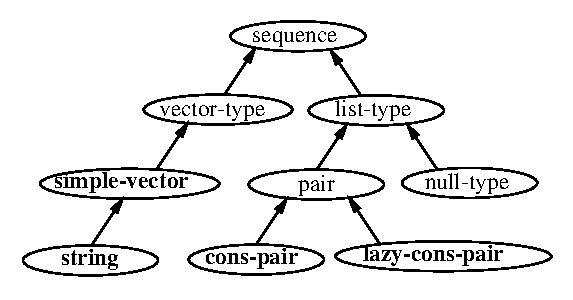
\includegraphics{seqhier}
\caption{The sequence type hierarchy.  Abstract types are in plain face
and instantiable ones in bold.} \label{fig:seqhier}
\end{figure}

\section{Type Predicates}

\pr{sequence?}{object}
\pr{vector?}{object}
\pr{string?}{object}
\pr{list?}{object}
\pr{pair?}{object}
\pr{null?}{object}
\pr{atom?}{object}


\section{Sequence Operations}

These operations work on all sequences.

\op{length}{list}
\lo{nth}{list n}
\lo{last}{list}
\lo{tail}{list n}
\op{copy}{sequence}

\op{append}{sequence1 sequence2}
\doc{Returns a sequence of the type of \emph{sequence1}.  One slight
bug is that one may not pass \df{append} a first argument that's a
list and a second that's not.  This may be fixed in the future.  All
other combinations should work correctly.}
\op{append\protect\bang}{sequence1 sequence2}
\doc{Most sequences have immutable lengths, and hence are not
appropriate arguments to \df{append\protect\bang}.  The major exception is lists.
The same bug is present here as in \df{append}.}

\op{reverse}{sequence}
\op{reverse\protect\bang}{sequence}

Some mapping operations are also applicable to sequences, and are
documented in Section~\ref{sec:controlmap}.

\section{Vector Constructors}

\op{vector}{\dt objects}
\doc{Returns a \df{simple-vector} containings \emph{objects}.}
\makin{simple-vector}{length}
\coercer{simple-vector}{sequence}


\section{List Constructors}

\op{list}{\dt objects}
\makin{list-type}{length fill-value}
\coercer{list-type}{sequence}
\op{cons}{object1 object2}
\makin{lazy-cons-pair}{car-thunk cdr-thunk}
\mc{lcons}{car-form cdr-form}
\doc{\macdef{}{(make lazy-cons-pair (lambda () \emph{car-form}) (lambda
() \emph{cdr-form}))}}


\section{List Accessors}

\lo{car}{pair}
\lo{cdr}{pair}
\lo{c$[$ad$]^{*}$r}{pair}
\doc{Actually these are only provided for up to four \texttt{a}'s and
\texttt{d}'s.  If you think you need more, you should probably be
defining accessor functions or using \df{nth} or perhaps
\df{destructure}.}
\lo{last-pair}{pair}
\doc{Takes successive \df{cdr}'s of \emph{pair} until it finds a pair
whose \df{cdr} is not a pair, which it returns.  \evto{(last-pair '(a
b c))}{(c)}.  \evto{(last-pair '(a b c . d))}{(c . d)}.}

\mc{destructure}{template structure \dt body}
\doc{This is for destructuring lists, and is sort of the inverse of
backquote.  \emph{Template} is a possibly nested list of variables.
These variables are bound to the corresponding values of 
\emph{structure} while \emph{body} is evaluated.  For instance,
\macdef{(destructure (a (b) . c) x (foo a b c))}{(let ((a (car x))(b
(caadr x))(c (cddr x))) (foo a b c))}.  It is guaranteed that 
\emph{structure} will be evaluated only once.  We note that \df{destructure}
typically generates more efficient code than the corresponding code
one might typically write.

If there is a position in \emph{template} that should be ignored, one
can place a \df{\#t} there.  For convenience and compatiblity with
\df{destructure*}, positions in \emph{template} containing \df{()},
\df{\#f} and \texttt{(quote \emph{x})} are also ignored.}

\mc{destructure*}{template structure \dt body}
\doc{This is just like \df{destructure} except that an error is
signaled if \emph{structure} doesn't precisely match \emph{template}.
Positions containing \df{\#f} and \df{()} are required to match
literally.  Positions containing \texttt{(quote \emph{x})} are required to
match \emph{x} literally, where \emph{x} is not evaluated.  As with
\df{destructure}, positions containing \df{\#t} are ignored.

\df{destructure*} is particularly useful in macro expanders where it
can do much of the syntax checking automatically.}

\mc{destructure**}{structure \lpar{}template \dt body\rpar ...
[\lpar{}\texttt{otherwise} \dt nomatch-body\rpar]}
\doc{This is just like \df{destructure*} except that, when one
template does not match, the next in line is considered.  If none
match than the OTHERWISE one does; if no otherwise clause is present,
an error is signaled.}


\section{Lists as Sets}

\op{mem}{predicate object list}
\doc{Returns the first tail of \emph{list} whose \df{car} equals 
\emph{object} according to \emph{predicate}.}

\op{memq}{object list}
\op{del}{predicate object list}
\op{delq}{object list}
\op{del\protect\bang}{predicate object list}
\op{delq\protect\bang}{object list}



\section{Lists as Associations}

\op{ass}{predicate object list}
\op{assq}{object list}
\so{cdr-ass}{predicate object list}
\so{cdr-assq}{object list}



\section{Lists as Stacks}

\mc{push}{location object}
\mc{pop}{location}

% This file is part of Oaklisp.
%
% This program is free software; you can redistribute it and/or modify
% it under the terms of the GNU General Public License as published by
% the Free Software Foundation; either version 2 of the License, or
% (at your option) any later version.
%
% This program is distributed in the hope that it will be useful,
% but WITHOUT ANY WARRANTY; without even the implied warranty of
% MERCHANTABILITY or FITNESS FOR A PARTICULAR PURPOSE.  See the
% GNU General Public License for more details.
%
% The GNU GPL is available at http://www.gnu.org/licenses/gpl.html
% or from the Free Software Foundation, 59 Temple Place - Suite 330,
% Boston, MA 02111-1307, USA


\chapter{Numbers} \label{numbers}

\index{\texttt{number}} \index{\texttt{real}} \index{\texttt{complex}}
\index{\texttt{rational}} \index{\texttt{float}} \index{\texttt{integer}}
\index{\texttt{fraction}} \index{\texttt{fixnum}} \index{\texttt{bignum}}

\begin{figure}[h]
\[ \myepsfbox{numhier.ips} \]
\caption{The numeric type hierarchy.  Abstract types are in plain face
and instantiable ones in bold.  Floating point numbers are not
implemented.} \label{fig:numhier}
\end{figure}

\section{Arithmetic}

\op{+}{\dt numbers}
\op{1+}{n}
\op{-}{n1 n2 \dt numbers}
\op{-}{n}
\op{*}{\dt numbers}
\op{/}{n1 n2}
\op{quotient}{n1 n2}
\op{modulo}{n1 n2}
\op{abs}{n1}
\op{max}{n1 n2}
\op{min}{n1 n2}
\op{expt}{n1 n2}


\section{Comparison}

\op{=}{n1 n2}
\op{{\protect\bang}=}{n1 n2}
\op{<}{n1 n2}
\op{>}{n1 n2}
\op{<=}{n1 n2}
\op{>=}{n1 n2}


\section{Predicates}

\pr{zero?}{n}
\pr{negative?}{n}
\pr{positive?}{n}
\pr{even?}{n}
\pr{odd?}{n}
\pr{factor?}{n1 n2}


\section{Rounding}

These operations should work on any subtype of \df{real}.

\op{floor}{x}
\doc{Returns the largest integer less than or equal to \emph{x}.}

\op{ceiling}{x}
\doc{Returns the smallest integer greater than or equal to \emph{x}.}

\op{truncate}{x}
\doc{Could be defined \texttt{(if (negative? x) (ceiling x) (floor x))}.}

\op{round}{x}
\doc{Returns nearest integer to \emph{x}.  Ties are broken by rounding
to an even number.}

\section{Bitwise Logical Operations}

These operations are only defined for integers.

\op{ash-left}{i amount}
\op{ash-right}{i amount}
\op{rot-left}{i amount}
\op{rot-right}{i amount}
\op{bit-not}{i}
\op{bit-and}{i1 i2}
\op{bit-or}{i1 i2}
\op{bit-nor}{i1 i2}
\op{bit-xor}{i1 i2}
\op{bit-nand}{i1 i2}
\op{bit-andca}{i1 i2}
\op{bit-equiv}{i1 i2}


\section{Accessing Components}

\op{numerator}{rational}
\op{denominator}{rational}

\op{real-part}{number}
\op{imag-part}{number}

% This file is part of Oaklisp.
%
% This program is free software; you can redistribute it and/or modify
% it under the terms of the GNU General Public License as published by
% the Free Software Foundation; either version 2 of the License, or
% (at your option) any later version.
%
% This program is distributed in the hope that it will be useful,
% but WITHOUT ANY WARRANTY; without even the implied warranty of
% MERCHANTABILITY or FITNESS FOR A PARTICULAR PURPOSE.  See the
% GNU General Public License for more details.
%
% The GNU GPL is available at http://www.gnu.org/licenses/gpl.html
% or from the Free Software Foundation, 59 Temple Place - Suite 330,
% Boston, MA 02111-1307, USA


\chapter{Input and Output}

\section{Streams and Files}

Streams are the tokens through which interaction with the outside
world occurs.  Although streams are primarily used for reading and
writing to files, they have found a number of internal uses.

\ty{stream}
\doc{The supertype of all streams.}

\ty{input-stream}
\doc{This is an abstract type.  Instantiable subtypes must define
methods for the \df{really-read-char} operation.}

\op{read-char}{input-stream}
\doc{Return a character, or \df{the-eof-token} if we've already read
the last character in the stream.}

\op{unread-char}{input-stream character}
\doc{Puts \emph{character} back into \emph{input-stream}.  One can only
put one character back, and it must be the last character read.}

\op{peek-char}{input-stream}
\doc{Equivalent to \texttt{(let ((c (read-char \emph{input-stream})))
(unread-char \emph{input-stream} c) c)}.}

\ob{the-eof-token}
\doc{This distinguished object is returned to indicate that one has
read past the end of the file.}


\ty{output-stream}
\doc{This is an abstract type.  Instantiable subtypes must define
methods for the \df{write-char} operation.}

\op{write-char}{output-stream character}

\op{newline}{output-stream}
\doc{Outputs a carriage return to \emph{output-stream}.}
\op{freshline}{output-stream}
\doc{Ensures that \emph{output-stream} is at the beginning of a line.}

\op{flush}{output-stream}
\doc{Flushes any buffered output.}

\op{interactive?}{stream}
\doc{Returns true if and only if \emph{stream} is connected to the
user.  This is used to check if an end of file condition on the
control stream is really an end of file or if the user just typed
control-D.}

\so{position}{stream}
\doc{Returns the position we are at within \emph{stream}.  By setting
this, one can get back to a previous position.}

\op{write-string}{string output-stream}
\doc{Writes the characters of \emph{string} to \emph{stream}.}

\mc{with-open-file}{\lpar variable filename \dt options\rpar \dt body}
\doc{Binds \emph{variable} to a stream which is connected to the file
with the name \emph{filename}.  \emph{Options} is not evaluated, and
describes how \emph{filename} should be opened.  Possible symbols
include \df{in} for input, \df{out} for output, and \df{append} for
output with position set to the end of the file.  The \df{ugly} option
can be added to either \df{out} or \df{append} if the user doesn't
mind poor formating, as in files meant to be read only by other
programs.  The opened stream will be closed when the
\df{with-open-file} is exited, even upon abnormal exit.  \textbf{Note:}
the stream is not reopened upon abnormal entry, but this may be
changed in future versions of the system.}

\mc{with-input-from-string}{\lpar variable sequence\rpar \dt body}
\doc{Binds \emph{variable} to an input stream whose contents are the
characters of \emph{sequence}.  Although \emph{sequence} is usually a
string, this will work correctly for any sequence type.}

\makin{string-output-stream}{}
\doc{These save all their output and return it as a string in response
to the \dfcoer{string} operation.}



\section{Reading}

Oaklisp has an industrial strength reader, replete with nonterminating
macro characters and descriptive error messages.  List syntax is not
described below; read some other lisp manual.  Our reader is modeled
after the Common Lisp reader, so we emphasize differences with the
Common Lisp reader below.

\op{read}{input-stream}
\doc{Returns a lisp object read from \emph{stream}.  This is sensitive
to a large number of factors detailed below.}

\ob{standard-read-table}
\doc{This holds the read table for usual lisp syntax.  The \df{nth}
operation can be used to get and set elements of read tables, which
are indexed by characters.  Potential entries are \df{whitespace},
\df{constituent}, \df{single-escape}, \df{illegal},
\emph{\lpar\df{terminating-macro} \dt operation\rpar}, and
\emph{\lpar\df{nonterminating-macro} \dt operation\rpar}.}

\op{skip-whitespace}{input-stream}
\doc{Reads characters from \emph{input-stream} until the next character
is not whitespace.}

The reader is not sensitive to the case of macro characters.

\op{define-macro-char}{character operation}
\doc{Defines \emph{character} to be a reader macro in
\df{standard-read-table}.  When \emph{character} is encountered by the
reader, \emph{operation} is called with two arguments, the stream and
the character that was read.}

\op{define-nonterminating-macro-char}{character operation}
\doc{Just like \df{define-macro-char} except that the macro is not
triggered if \emph{character} is read inside a token.}

There are a number of ``quotelike'' macro characters present for the
convenience of the user.

\begin{center}
\begin{tabular}{cl}
\emph{macro character} & \emph{symbol} \\\hline
\texttt{'} & \df{quote} \\
\texttt{`} & \df{quasiquote} \\
\texttt{control-v} & \df{fluid} \\
\texttt{control-y} & \df{coercer} \\
\texttt{,@} & \df{unquote-splicing} \\
\texttt{,} & \df{unquote}
\end{tabular}
\end{center}

\op{define-quotelike-macro-char}{character object}
\begin{docenv}
Makes \emph{character} a terminating macro which returns a list of
\emph{object} and the next thing read.  This also arranges for the printer
to print using analogous syntax.  For instance, the quote syntax is
defined with the line \texttt{(define-quotelike-macro-char
\texttt{\#'} 'quote)} in the system internals.
\end{docenv}

\ob{the-unread-object}
\doc{When a reader macro returns this, the reader takes it to mean
that nothing at all was read.  For instance, the reader macro for
\texttt{;} reads the remainder of the line and returns this.}

The character \texttt{[} is used to read lists in the same way that
\texttt{(} is, except that \texttt{[} must be matched by a \texttt{]}.
This is mostly for compatiblity with code written at the University of
Indiana.

Since there are no packages in Oaklisp, the \texttt{:} character is
treated like any other constituent.

Most of the Common Lisp hash reader macros are supported.  For
instance, the character object representing \texttt{a} is read
\texttt{\#$\backslash$a}.  Many special characters have long names, such as
\texttt{\#$\backslash$space}.

\op{define-hash-macro-char}{character operation}
\doc{Defines \emph{character} to be a hash reader macro character.
\emph{Operation} should take three arguments: a stream, the character,
and the numeric argument that was between the hash and the character,
\df{\#f} if none was passed.}

There are many hash reader macro characters, including \df{\#o},
\df{\#x}, \df{\#d}, \df{\#b} and \df{\#c} for octal, hexidecimal,
decimal, binary and complex numbers, respectively.  The syntax
\texttt{\#\emph{n}r\emph{xxx}} is used to read \emph{xxx} in base \emph{n}.
\texttt{\#(\ldots)} is used for reading vectors.  The \texttt{\#|} macro
comments out text until a matching \texttt{|\#}, with proper nesting.  As
described in Section~\ref{sec:truths}, \df{\#t} and \df{\#f} are read
as the canonical true and false values, respectively.

The \texttt{\#[symbol "\ldots"]} syntax can be used to read arbitrary
characters, although the \texttt{|$\ldots$|} construction is prefered.
Analogous constructors can be added with the settable operation
\df{hash-bracket-option}.

\fv{input-base}
\doc{The radix in which numbers will be read.}

\fv{features}
\doc{A list of ``features'' present in the current implementation,
used by the \df{\#+} and \df{\#-} reader macros.  Testable and
settable with the \df{feature?} settable operation.  It is guaranteed
that the \df{oaklisp} and \df{scheme} features will be present in any
implementation of Oaklisp.}

\fv{current-locale}
\doc{The \df{\#.} macro evaluates its argument in this locale.}

\fv{read-suppress}
\doc{This is true when what is being read will just be ignored, and
indicates to the reader that it shouldn't go to the trouble of
interpreting the meaning of complex tokens or anything like that.}



\section{Printing}

The printer is pretty heavy duty, but has no facilities for printing
circular objects.

\op{format}{stream control-string \dt args}
\doc{This is very similar to the Common Lisp \df{format} function, and
is the usual way for users to print things.

\emph{Stream} is permitted to be \df{\#t} to indicate that output
should be sent to the standard output, and \df{\#f} to indicate that
the output should be bundled up into a string and returned.

Characters in {control-string} are printed directly, except for the
\texttt{\~} character which indicates that some action should be taken.
The \texttt{\~} may be followed by a number or by a \texttt{:} or
\texttt{@}, which vary the action that would normally be taken in some
way.

Currently defined \texttt{\~} characters and their associated actions
are:

\begin{itemize}
\item[\texttt{A}] Print and argument with \dffl{print-escape} bound to
	\df{\#f}.

\item[\texttt{\~}] Print a \texttt{\~}.

\item[\texttt{\%}] Do a \df{newline}.

\item[\texttt{\&}] Do a \df{freshline}.

\item[\texttt{S}] Print an argument with \dffl{print-escape} bount to \df{\#t}.

\item[\texttt{B}] Print an argument in binary.

\item[\texttt{D}] Print an argument in decimal.

\item[\texttt{O}] Print an argument in octal.

\item[\texttt{X}] Print an argument in hex.

\item[\texttt{\emph{n}R}] Print an argument in base \emph{n}.

\item[\texttt{C}] Print an argument which is a character.

\item[\texttt{P}] Print an \texttt{s} if the argument is not 1.

\item[\texttt{!}] Print a weak pointer to the argument, preceded by an
expression which evaluates to the argument if \dffl{fancy-references}
is on.  This is used to print unique id's for objects without nice
printed representations, like operations.

\end{itemize}

A tilde followed by a newline is ignored; this construct is used for
making \emph{control-string} more readable by breaking it across lines.}


\op{print}{object stream}
\doc{Writes a representation of \emph{object} to \emph{stream}.  Users
are encouraged to add informative print methods for types they define.}

\op{define-simple-print-method}{type string}
\doc{Instructs the printer to include \emph{string} in the printed
representation of instances of \emph{type}.}

\fv{print-radix}
\doc{The radix in which numbers will be printed.  The default is ten.}

\fv{print-level}
\doc{The number of levels of list structure to be printed before the
printer abbreviates.  The default is \df{\#f}, meaning never abbreviate.}

\fv{print-length}
\doc{The number of elements of a list to be printed before the printer
abbreviates.  The default is \df{\#f}, meaning never abbreviate.}

\fv{print-escape}
\doc{This controls whether the printer tries to print things that are
easy for people to read, or ones that can be read back in to Oaklisp.
The default is \df{\#t}, meaning to maintain print/read consistency at
the expense of readability.}

\fv{symbol-slashification-style}
\doc{This controls the style of printing of symbols when they are
escaped.  See the implementation manual for details.}

\fv{fraction-display-style}
\doc{This can be either \df{normal}, \df{fancy} or \df{float}.  In
these cases, \texttt{(/ -5 3)} would print as either \texttt{-5/3},
\texttt{-1$\cdot$2/3} or \texttt{-1.6666666666}, respectively.}

\chapter{Miscellaneous} \label{misc}

\section{Tables}

The types are \df{generic-hash-table} and \df{eq-hash-table}.  The
access interface is \df{present?}, which returns a \df{pair} whose
\df{car} is the key and whose \df{cdr} is the associated value.  A
different interface to hash tables is provided by the T-style
\df{table-entry} operation which returns the associated value or
\df{\#f} if the key isn't in the table.  The setter of either
operation can be used to add, modify, and remove associations.

\makin{generic-hash-table}{key-hash-op equal-op}
\makin{eq-hash-table}{}

\so{present?}{table key}
\doc{Returns {\tt (\em key \dt val\tt)} pair, or \df{\#f} if not present.}

\so{table-entry}{table key}
\doc{Returns value indexed by {\em key} or \df{\#f} if not present.}




\section{Delays}

Oaklisp's delays are compatible with the facility defined in R3RS, but
extend those primitive facilities in two ways.  First, the system will
automatically force promises when appropriate.  For instance, {\tt (+
2 (delay 3))} does not signal an error; it returns {\tt 5}.
Similarly, delays are printed transparently, slightly violating
read/print consistency.  Secondly, the delay facility is user
extensible.  Users can create new kinds of delays that have special
protocols, for instance numeric delays that do not force themselves
upon arithmetic operations, but instead make more and more complicated
delays.


\sform{delay}{expression}
\doc{This immediately returns a {\em promise} for {\em expression},
without actually computing {\em expression}.  This promise does not
compute {\em expression} until it is forced, at which point it
returns the value of {\em expression}, computing it if it hasn't
already done so.}

\op{force}{x}
\doc{If {\em x} is a promise, it is forced to compute its value, which
is returned.  If {\em x} is not a promise, it itself is returned.}

\ty{promise}
\doc{This is the type of the objects returned by \df{delay}.}

\ty{forcible}
\doc{This is an abstract type, of which \df{promise} is a concrete
subtype.  Subtypes of \df{forcible} are expected to respond to the
\df{force} operation in a sensible fashion.  Oaklisp's system
internals sometimes force instances of \df{forcible} automatically,
for instance when sending them messages for which no appropriate
method can otherwise be found.}

\fv{forcible-print-magic}
\doc{Controls how delays are printed.  This is how {\tt (delay 'foo)}
would print under various settings of {\tt forcible-print-magic}.
\begin{center}
\begin{tabular}{|l|l|}\hline
value             & print style             \\ \hline
{\tt\#f}          & {\tt\#<DELAY 3462>}     \\
{\tt indicate}    & {\tt\#[DELAY FOO 3462]} \\
{\tt transparent} & {\tt FOO}               \\ \hline
\end{tabular}
\end{center}
The default is \df{transparent}.  A setting of \df{indicate} is more
instructive if you encounter odd behavior that might be due to
delays.}

% This file is part of Oaklisp.
%
% This program is free software; you can redistribute it and/or modify
% it under the terms of the GNU General Public License as published by
% the Free Software Foundation; either version 2 of the License, or
% (at your option) any later version.
%
% This program is distributed in the hope that it will be useful,
% but WITHOUT ANY WARRANTY; without even the implied warranty of
% MERCHANTABILITY or FITNESS FOR A PARTICULAR PURPOSE.  See the
% GNU General Public License for more details.
%
% The GNU GPL is available at http://www.gnu.org/licenses/gpl.html
% or from the Free Software Foundation, 59 Temple Place - Suite 330,
% Boston, MA 02111-1307, USA


\chapter{User Interface} \label{user}

The Oaklisp user interface currently consists of a read-eval-print
loop and a simple debugging facility.

Errors land the user into a recursive evaluation loop in which special
restart handlers are available.  Our implementation includes
mechanisms for inspecting objects and tracing function calls.


\section{The Top Level Environment}

All expressions must be evaluated with respect to a particular naming
environment.  The read-eval-print loop uses the locale specified by
the fluid variable \df{current-locale}.  The Oaklisp system boots up
with this variable bound to \df{user-locale}.  Other useful name
spaces are \df{scheme-locale}, \df{system-locale}, and
\df{compiler-locale}.

Several fluid variables are used to keep a short history of the
dialogue conducted by the top level evaluator.  The most useful of
these is \dffl{*}, which contains the value produced by the most
recent user expression.  The value of this variable is rolled back
into \dffl{**} and then into \dffl{***} to provide access to the three
most recent values.  Similarly, there are three copies of \dffl{+} and
\dffl{?} that provide access to recent expressions that were read in
and to their form after macro expansion.

The switch \dffl{fancy-references} controls the printing of anonymous
objects.  When this switch is turned off, an object usually prints out
something like this: \texttt{\#<op 806>}.  This format indicates the type
of the object, and provides a weak pointer that can be derefenced with
\df{object-unhash} to get the object.  When the
\dffl{fancy-references} switch is turned on, the printer attempts to
generate an expression that will evaluate to the object in the current
locale.  For example, the above operation might print out as \texttt{\#<op
(setter car) 806>}.  The default value for this switch is
\df{\#f}, but it is briefly switched on by \df{describe}.

Two more fluid variables that are frequently used at the top level are
\dffl{print-length} and \dffl{print-level}, which are normally set to
small integer values in order to abbreviate the printing of long
lists, but which can be set to \df{\#f} in order to enable exhaustive
printing.

%%
%
% The read-eval-print loop uses the \df{eval} function to perform the
% actual evaluation of expressions.  The \df{eval} function in turn
% calls one of several functionally equivalent evaluation functions in
% our implementation: \df{interpreter-eval}, \df{compiler-eval}, and
% \df{hybrid-eval}.  The variable \dffl{top-level-evaluator}
% specifies which one should be used.  \df{hybrid-eval} is the default
% value in worlds that contain the compiler.  This evaluator minimizes
% top level latency by only using the compiler for expressions that
% contain \df{add-method} forms.
%
%


\section{Miscellaneous Functions}

There are some other very useful functions that are part of the user
interface.

\op{apropos}{word [place]}
\doc{Returns either variables or symbols containing \emph{word},
depending on \emph{place}, which can be a locale or \df{symbol-table}.
\emph{place} defaults to \dffl{current-locale}.}

\oop{\%gc}
\doc{Collect garbage.  This does not collect garbage in ``static
space,'' but it is exceedingly unlikely that there is any there.}
\oop{\%full-gc}
\doc{Collect more garbage.  This does collect garbage from ``static
space,'' but more importantly, it put everything not freed into static
space, so it need not be transported in future normal garbage
collections.}



\section{Debugging}


The following special forms can be used to trace the
execution of an operation.

\sform{trace-variable-in}{global-var}
\doc{Puts a trace on the operation stored in \emph{global-var}, causing
a message to be printed every time the operation is called.}

\sform{trace-variable-out}{global-var}
\doc{Puts a trace on the operation stored in \emph{global-var}, causing
a message to be printed every time a call to the operation returns.}

\sform{trace-variable-in-out}{global-var}
\sform{untrace-variable}{global-var}


Objects can be examined in detail with the \df{describe}
function, which prints the object and its type with
\dffl{fancy-references} turned on, followed by the object's
internal state.  The internal state is organized as instance-variable
blocks from the object's various component types.  An object's
internal state usually contains anonymous objects whose printed
representation includes weak pointers which can be dereferenced using
\df{object-unhash}.  Together, \df{describe} and \df{object-unhash}
constitute a simple but effective inspector.

To simplify this process \texttt{describe} applied to an integer which is
the \texttt{object-hash} of some object will describe that object.  In
other words, \texttt{describe} can be applied to the numeric ID in an
object's printed representation.

\op{describe}{object}
\doc{Prints out lots of stuff about \emph{object}.}

\op{object-unhash}{i}
\doc{Dereferences the weak pointer \emph{i}.}


When an error occurs in our implementation of Oaklisp, the
user is thrown into a recursive evaluation loop whose dynamic context
is nested inside that of the error.  Several restart handlers are
typically available in a recursive evaluation loop, and the \df{ret}
function is the mechanism for invoking one of these handlers.
\df{call/cc} can be used to preserve an error context when it might
be useful to restart the computation at a later time.


\op{ret}{n \dt args}
\doc{Invokes restart handler \emph{n}, as specified by the list of
handlers printed out by a subordinate evaluation loop.  \texttt{(ret 0)},
which returns control to the top level evaluation loop, is always in
effect.}

The following dialogue with Oaklisp illustrates some of these
points.

\begin{verbatim}
Oaklisp 1.0  - (C) 1987 Barak A. Pearlmutter and Kevin J. Lang.
Oaklisp evaluation loop.
  Active handlers:
  0: Return to top level.

> (with-open-file (inf "fone.nums" in) (car (read inf)))

Error: Error opening "fone.nums" for reading.
Oaklisp evaluation loop.
  Active handlers:
  0: Return to top level.
  1: Retry opening file (argument for different file name).
  2: Return to debugger level 1.

>> (call/cc identity)                ;get error context.

>> (set foo (fluid *))               ;stash it away.

>> (ret 0)                           ;back to top level.

   Invoking handler Return to top level..

> (describe foo)                    ;inspect continuation.

#<Op FOO 798> is of type #<Type OPERATION 801>.

 from #<Type 801>:
  LAMBDA? : #<Object 802>           ;what's this thing?
  CACHE-TYPE : 0
  CACHE-METHOD : 0
  CACHE-TYPE-OFFSET : 0

> (describe (object-unhash 802))

#<Object 802> is of type #<Type %METHOD 803>.

 from #<Type 803>:
  THE-CODE : #<VLmixin 804>
  THE-ENVIRONMENT : #<VLmixin 805>

> (foo 0)                    ;re-enter error context.

>> (ret 1 "phone.nums")      ;resume computation

   Invoking handler Retry opening the file ...

268-7598                     ;got that phone number!

> (exit)

Oaklisp stopped itself...
\end{verbatim}

Using the error system effectively is an important part of providing
the user with a helpful interface.  Details on the error system can be
found in Section~\ref{errors}.


\nocite{OAKLANG88}
\nocite{CLOOPS}
\nocite{FLAVORS2}
\nocite{MVC}
\nocite{R3RS}
\nocite{SCHEME-DECLARATIVE}
\nocite{SCHEME-PAP}
\nocite{SNYDER86}
\nocite{T}
\nocite{T-MAN}
\nocite{OAK-PAP}
\nocite{3LISP}
\nocite{FLAVORS1}
\nocite{CLtL}
\nocite{MULTILISP85}
\nocite{ACTORS78}
\nocite{CITY-TRASH}
\nocite{PEARLMUTTER-LANG90A}
\nocite{PEARLMUTTER99}

\bibliography{../oakman}

\printindex

\end{document}
